%**************************************************************
\subsubsection{Package it.tecsen.smacs.view}
\label{subsubsec:it-tecsen-smacs-view}

\begin{figure}[!h]
  \centering 
  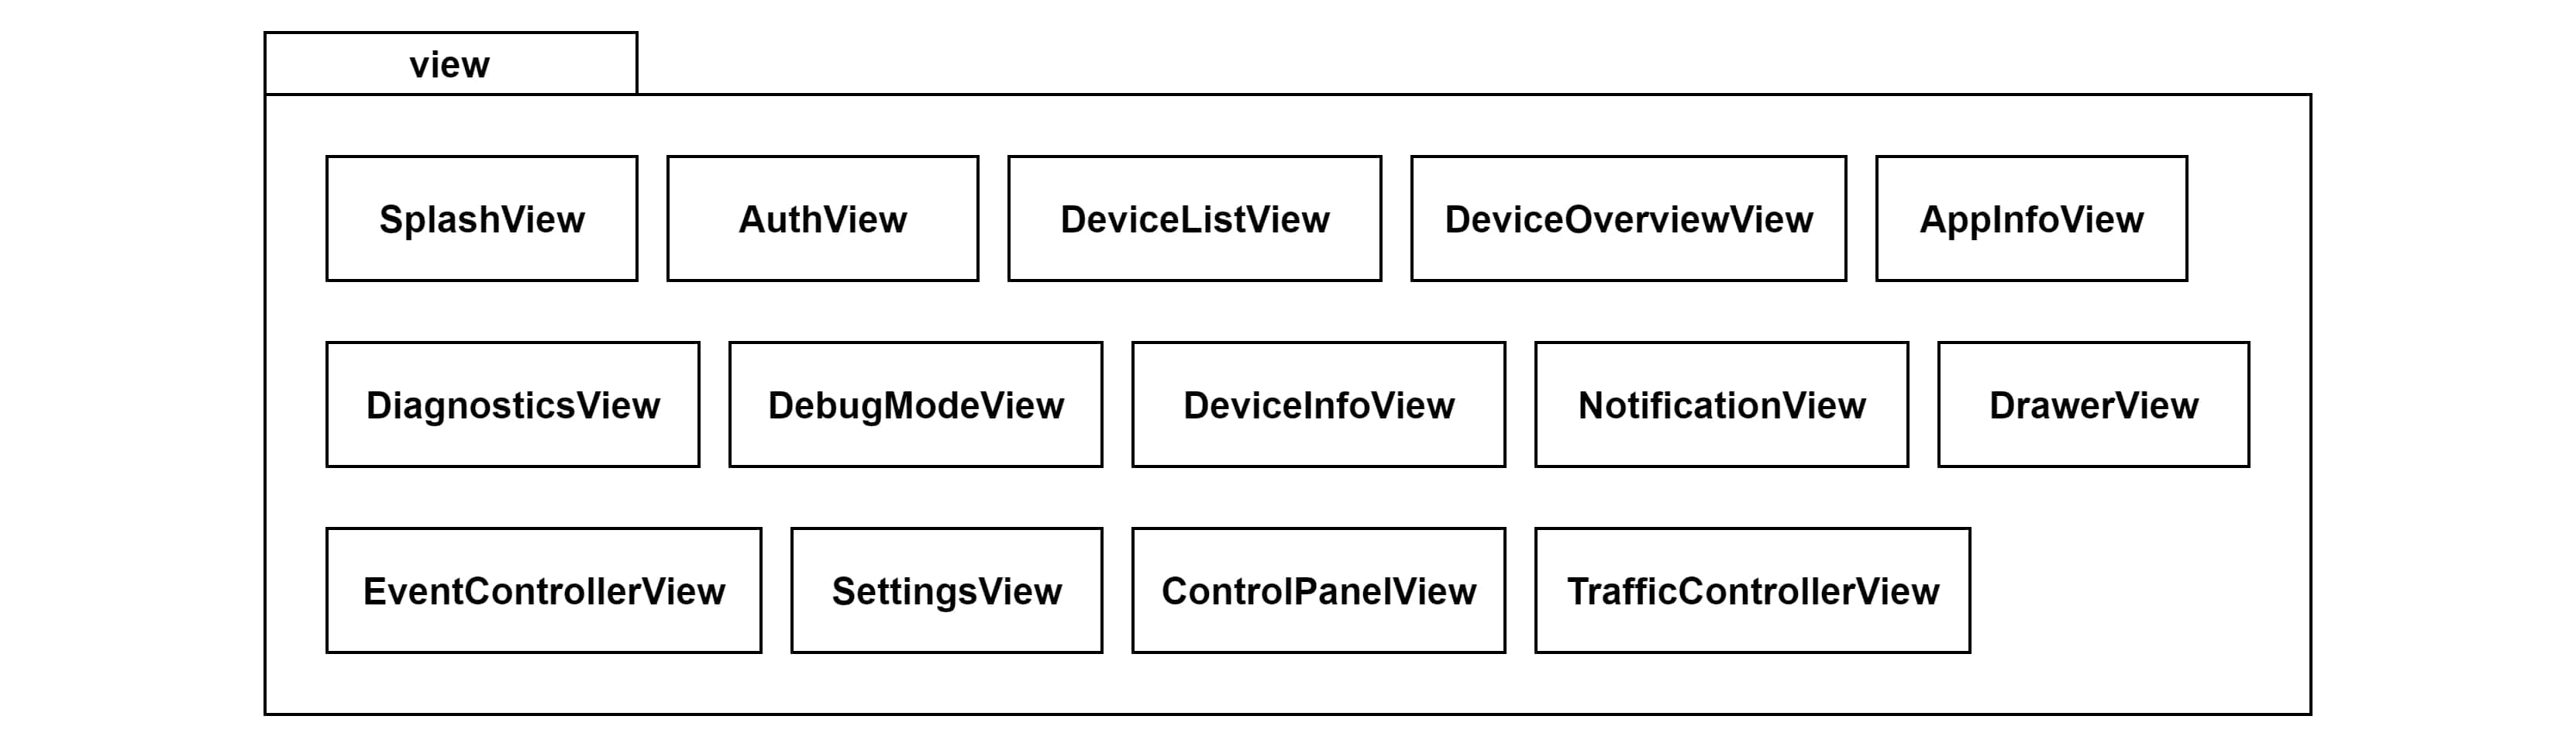
\includegraphics[width=1.0\columnwidth]{capitolo-6/organizzazione-package/view} 
  \caption{Diagramma del package \texttt{it.tecsen.smacs.view}}
\end{figure}
In questo package vi sono tutte le classi che implementano i widget che visualizzano il contenuto per soddisfare i casi d'uso raccolti.\\
Ogni classe implementa uno o più casi d'uso, disponibili per la consultazione nell'appendice "\hyperref[cap:analisi-dei-requisiti]{Analisi dei requisiti}".\\
In particolare:
{
\renewcommand{\arraystretch}{1.5}
\begin{longtable}{|c|c|}
    \hline
    \textbf{Classe (widget)} & \textbf{Caso (e sotto-casi) d'uso implementati} \\\hline
    \endhead
    SplashView & UC01\\\hline
    AuthView & UC02 \\\hline
    DeviceListView & UC03 \\\hline
    DeviceOverviewView & UC04.1, UC04.2, UC04.3, UC04.4, UC04.5, UC05 \\\hline
    DiagnosticsView & UC04.5, UC04.6, UC07.3 \\\hline
    ControlPanelView & UC04.5, UC07.1, UC07.2, UC07.4 \\\hline
    TrafficControllerView & UC04 e UC07 (sotto-casi esclusi), UC04.7, UC09, UC10 \\\hline
    DeviceInfoView & UC06 \\\hline
    EventControllerView & UC08 \\\hline
    NotificationView & UC11 \\\hline
    SettingsView & UC12 \\\hline
    AppInfoView & UC13 \\\hline
    DebugModeView & UC14 \\\hline
    DrawerView & UC15 \\\hline
    \caption{Correlazione fra classi del package \texttt{view} e casi d'uso implementati}
\end{longtable}
}